\documentclass[ecp,tc,english]{infufrgs}

\usepackage[utf8]{inputenc}
\usepackage{graphicx}
\usepackage{booktabs}
\usepackage{rotating}     
\usepackage{array}
\usepackage{amsmath}
\usepackage{microtype}
\setlength{\emergencystretch}{2em}

% -------------------- Metadados --------------------
\title{Assessing the Impact of Data Leakage in Machine Learning Pipelines for Regression Tasks}
\translatedtitle{Avaliacao do Impacto do Vazamento de Dados em Pipelines de Aprendizado de Maquina para Tarefas de Regressao}

\author{Piacini}{Vinicius}

\advisor[Profa.~Dra.]{Recamonde-Mendoza}{Mariana}

% Data da defesa (padrao: mes e ano atuais)
% \date{dezembro}{2026}

% -------------------- Palavras-chave --------------------
\keyword{Data Leakage}
\keyword{Regression Analysis}
\keyword{Machine Learning Evaluation}
\keyword{Model Assessment}

\translatedkeyword{Vazamento de Dados}
\translatedkeyword{Analise de Regressao}
\translatedkeyword{Avaliacao de Aprendizado de Maquina}
\translatedkeyword{Estimativa de Desempenho}

\begin{document}

\maketitle

% -------------------- Elementos pre-textuais --------------------
% \begin{dedicatoria}
%   ...
% \end{dedicatoria}

% \begin{agradecimentos}
%   ...
% \end{agradecimentos}

\begin{abstract}
Reliable estimates of generalization performance are essential to assess machine
learning models, but they depend on a strict separation between the data used to
build a model and the data used to evaluate it. Data leakage breaks this
separation and may produce overly optimistic results without any visible sign.
Although the problem is widely discussed, there is little systematic evidence on
how different sources of leakage affect regression models. This work
investigates leakage introduced at four steps of a machine learning pipeline:
normalization, missing value imputation, feature selection, and hyperparameter
tuning. Using a paired design, leakage-free and leakage-prone pipelines were
evaluated on the same data partitions for 21 regression data sets from the Penn
Machine Learning Benchmarks and five algorithms (linear regression, k-nearest
neighbors, decision trees, random forests, and support vector regression),
totaling 11,340 paired comparisons analyzed with $R^2$, RMSE, and non-parametric
statistical tests. % Resultados omitidos nesta versao (capitulos 5 e 6 em construcao).
\end{abstract}

\begin{translatedabstract}
Estimativas confi\'aveis do desempenho de generaliza\c{c}\~ao s\~ao essenciais para
avaliar modelos de aprendizado de m\'aquina, mas dependem de uma separa\c{c}\~ao
estrita entre os dados usados para construir um modelo e os dados usados para
avali\'a-lo. O vazamento de dados rompe essa separa\c{c}\~ao e pode produzir
resultados excessivamente otimistas sem nenhum sinal vis\'ivel. Embora o
problema seja amplamente discutido, h\'a pouca evid\^encia sistem\'atica sobre
como diferentes fontes de vazamento afetam modelos de regress\~ao. Este trabalho
investiga o vazamento introduzido em quatro etapas de um pipeline de
aprendizado de m\'aquina: normaliza\c{c}\~ao, imputa\c{c}\~ao de valores
faltantes, sele\c{c}\~ao de atributos e ajuste de hiperpar\^ametros. Com um
desenho pareado, pipelines com e sem vazamento foram avaliados sobre as mesmas
parti\c{c}\~oes de dados em 21 conjuntos de dados de regress\~ao do Penn Machine
Learning Benchmarks e cinco algoritmos (regress\~ao linear, k vizinhos mais
pr\'oximos, \'arvores de decis\~ao, florestas aleat\'orias e regress\~ao por
vetores de suporte), totalizando 11.340 compara\c{c}\~oes pareadas analisadas
com $R^2$, RMSE e testes estat\'isticos n\~ao param\'etricos. % Resultados omitidos nesta versao (capitulos 5 e 6 em construcao).
\end{translatedabstract}

\tableofcontents
\listoffigures
\listoftables

\begin{listofabbrv}{RMSE}
  \item[CV]   Cross-Validation
  \item[DL]   Data Leakage
  \item[DT]   Decision Tree
  \item[KNN]  K-Nearest Neighbors
  \item[LR]   Linear Regression
  \item[MAE]  Mean Absolute Error
  \item[MAR]  Missing At Random
  \item[MCAR] Missing Completely At Random
  \item[ML]   Machine Learning
  \item[MNAR] Missing Not At Random
  \item[MSE]  Mean Squared Error
  \item[OLS]  Ordinary Least Squares
  \item[PMLB] Penn Machine Learning Benchmarks
  \item[RBF]  Radial Basis Function
  \item[RF]   Random Forest
  \item[RMSE] Root Mean Squared Error
  \item[SVR]  Support Vector Regression
\end{listofabbrv}

% -------------------- Elementos textuais --------------------
\chapter{Introduction}
\label{cap:introducao}

Machine Learning (ML) models have become central to scientific research and
industrial applications, supporting decision-making processes in domains such as
healthcare, finance, engineering, and environmental sciences. As predictive
models are increasingly deployed in high-stakes settings, the reliable estimation
of their generalization performance becomes essential. Rigorous evaluation
protocols are required not only for comparing competing methods, but also to
ensure that reported results accurately reflect how models behave on previously
unseen data. However, when the process of training and validating ML models is
not conducted correctly from a methodological point of view, the reported
performance may diverge substantially from the model's real predictive
capability. \citeonline{kapoor2023} argue that such methodological issues are
widespread in ML-based scientific research, contributing to what has been
described as a reproducibility crisis in machine-learning-based science.

Among the factors that compromise evaluation reliability, data leakage (DL) is
one of the most critical and persistent. Data leakage is defined as the
contamination of the training process with privileged information from the
independent validation or test set, to which the algorithm should not have access
during model development \cite{kaufman2012}. Under a broader interpretation
\cite{kapoor2023}, leakage extends beyond direct train-test overlap and includes
more subtle methodological flaws, such as applying normalization using statistics
computed over the entire data set, imputing missing values before data splitting,
performing feature selection with information from both training and validation
sets, or tuning hyperparameters in a way that indirectly incorporates evaluation
data. Although these practices are frequently introduced unintentionally, they
bias performance estimates and may produce misleading conclusions about model
quality.

The relevance of the problem has motivated a growing body of research focused on
the characterization, detection, and mitigation of leakage, including formal
definitions \cite{kaufman2012}, taxonomies of leakage types \cite{kapoor2023},
static code analysis approaches \cite{drobnjakovic2022,yang2022}, and
domain-specific guidelines \cite{bernett2024,apicella2024}. Empirical
demonstrations of the phenomenon are comparatively scarcer, and the most
influential ones come from bioinformatics: \citeonline{ambroise2002} showed that
performing gene selection outside the cross-validation loop drives the estimated
error rate close to zero even on data with no real signal, and
\citeonline{varma2006} showed that the cross-validation error of a model whose
hyperparameters were themselves chosen by cross-validation is a significantly
biased estimate of the true error. These results, however, are confined to
classification and to a single application domain. More recently,
\citeonline{becker2023} conducted a systematic assessment of data leakage effects
on the performance estimates of ML classifiers across several data sets and
algorithms, showing that the magnitude of the distortion varies according to both
the learning algorithm and the pre-processing step in which the leakage
originates. Regression tasks, despite being equally susceptible to the same
methodological flaws, have not received an equivalent treatment, and it remains
unclear whether the patterns observed for classifiers transfer to continuous
prediction targets.

This work aims to address this gap by proposing a systematic and controlled study
of the effects of data leakage on the performance estimates of ML models
developed for regression tasks. The objective is to understand how different data
sets and learning algorithms are affected by each kind of pre-processing
contamination: normalization, missing values imputation, feature selection, and
hyperparameter optimization. For each of these steps, experiments contrast a
leakage-free pipeline with a leakage-prone counterpart under otherwise identical
conditions, using benchmark regression data sets obtained from the Penn Machine
Learning Benchmarks collection \cite{romano2022} and a diverse set of supervised
learning algorithms. By isolating each contamination mechanism, this work seeks
to quantify the magnitude and the variability of the performance inflation caused
by data leakage, and to investigate whether certain regression algorithms are
more sensitive to these distortions than others.

This work is organized as follows. Chapter~\ref{cap:fundamentacao} provides a
theoretical background, describing the key concepts for this work, including the
regression algorithms employed, the pre-processing and validation procedures
adopted, and the notion of data leakage. Chapter~\ref{cap:trabalhos} summarizes
existing efforts based on related works. Next, Chapter~\ref{cap:metodologia}
presents the methods used, including the selection of data and the experimental
methodology adopted for each contamination scenario. The experimental results are
unveiled in Chapter~\ref{cap:resultados}, alongside the research questions that
our work aimed to address. Finally, conclusions and possible future works are
presented in Chapter~\ref{cap:conclusao}.

\chapter{Theoretical Background}
\label{cap:fundamentacao}

This chapter presents the concepts that support the remainder of this work.
Section~\ref{sec:fund-regressao} defines the regression task and the metrics
used to evaluate regression models. Section~\ref{sec:fund-algoritmos} describes
the five learning algorithms adopted in the experiments.
Section~\ref{sec:fund-pipeline} presents the pipeline steps investigated in this
study and the procedures used to estimate model performance.
Section~\ref{sec:fund-vazamento} discusses how data leakage may arise in each of
these steps. Finally, Section~\ref{sec:fund-estatistica} describes the
statistical tests used in the analysis of the results.

\section{Regression and Its Evaluation}
\label{sec:fund-regressao}

In supervised learning, a model is trained from a set of instances for which the
expected output is known. Each instance is described by a vector of input
features $\mathbf{x}$ and is associated with an output value $y$, called the
target. The learning algorithm uses these instances to build a model capable of
predicting the target of new instances. When the target is categorical, the task
is called classification; when it is a continuous numerical value, such as the
price of a property or the body fat percentage of a person, the task is called
regression \cite{hastie2009}. This work addresses regression tasks only.

The purpose of a model is to make accurate predictions for instances that were
not available during training. A model that fits the training data very closely
may still perform poorly on new data, a phenomenon known as overfitting.
Therefore, model performance must be measured on data that were not used for
training, and the result is taken as an estimate of the model's generalization
performance, that is, of how it is expected to behave in practice.

In regression, the quality of a prediction is measured by its deviation from the
true value. Given $m$ evaluation instances with true values $y_i$ and predicted
values $\hat{y}_i$, the four metrics adopted in this work are defined as:

\begin{align}
  \text{MAE}  &= \frac{1}{m}\sum_{i=1}^{m} \lvert y_i - \hat{y}_i \rvert, \label{eq:mae}\\
  \text{MSE}  &= \frac{1}{m}\sum_{i=1}^{m} (y_i - \hat{y}_i)^2, \label{eq:mse}\\
  \text{RMSE} &= \sqrt{\text{MSE}}, \label{eq:rmse}\\
  R^2         &= 1 - \frac{\sum_{i=1}^{m} (y_i - \hat{y}_i)^2}{\sum_{i=1}^{m} (y_i - \bar{y})^2}, \label{eq:r2}
\end{align}

\noindent where $\bar{y}$ is the mean of the true values. The Mean Absolute Error
(MAE) is the average magnitude of the errors. The Mean Squared Error (MSE)
squares each error before averaging, so that large errors have a greater
influence on the result. The Root Mean Squared Error (RMSE) is the square root of
the MSE and is expressed in the same unit as the target, which makes it easier
to interpret. For these three metrics, lower values indicate better models.
However, they depend on the scale of the target: the same RMSE may represent a
small error for a target measured in thousands and a large error for a target
measured in units. Consequently, their values cannot be directly compared across
data sets.

The coefficient of determination ($R^2$) does not have this limitation. It
measures the proportion of the variance of the target that is explained by the
model, using as reference a baseline model that always predicts the mean of the
target. A value of 1 corresponds to perfect predictions, a value of 0 indicates
that the model performs as well as the baseline, and negative values indicate
that it performs worse than the baseline. Because it is independent of the scale
of the target, $R^2$ allows comparisons across data sets and is considered more
informative than the other metrics for this purpose \cite{chicco2021}. For this
reason, $R^2$ is the primary metric of this work, and RMSE is used as a
complementary metric.

\section{Regression Algorithms}
\label{sec:fund-algoritmos}

Five algorithms were considered in this work. They were selected because they
represent different learning approaches, which may lead to different
sensitivities to data leakage.

\subsection{Linear Regression}

Linear Regression (LR) models the target as a linear combination of the
features, $\hat{y} = \beta_0 + \beta_1 x_1 + \dots + \beta_d x_d$. The
coefficients $\beta_j$ are estimated by Ordinary Least Squares (OLS), which
minimizes the sum of the squared errors on the training data \cite{hastie2009}.
LR is simple, computationally efficient, and has no hyperparameters in its basic
form. A property of LR that is relevant to this work is that its predictions do
not change when a feature is shifted or multiplied by a constant, since the
corresponding coefficient is adjusted accordingly. Some variants impose
constraints on the coefficients, such as requiring all of them to be
non-negative, and these options can be treated as hyperparameters.

\subsection{K-Nearest Neighbors}

The K-Nearest Neighbors (KNN) algorithm is an instance-based method: it stores
the training data and predicts the target of a new instance as the average
target of the $K$ training instances closest to it \cite{cover1967,hastie2009}.
Its main hyperparameters are the number of neighbors $K$ and the distance
function used to measure the proximity between instances, such as the
Euclidean or the Manhattan distance. Since distances are computed directly from
the feature values, features with larger ranges have a greater influence on the
choice of the neighbors than features with smaller ranges. For this reason, KNN
is highly sensitive to the scale of the features.

\subsection{Decision Trees}

A Decision Tree (DT) recursively divides the feature space into regions. At each
node, the algorithm selects a feature and a threshold that split the training
instances into two groups, choosing the split that most reduces the error of the
predictions in the resulting groups. This process is repeated until a stopping
criterion is met, and the prediction of each terminal node, or leaf, is the mean
target of the training instances that reach it \cite{breiman1984}. Since each
split only compares a feature with a threshold, decision trees are not affected
by the scale of the features. However, a tree that grows without restrictions
tends to overfit the training data, so its complexity is usually controlled by
hyperparameters such as the maximum depth.

\subsection{Random Forests}

A Random Forest (RF) is an ensemble of decision trees whose predictions are
averaged \cite{breiman2001}. Each tree is trained on a bootstrap sample of the
training instances and, at each node, considers only a random subset of the
features. This randomness makes the trees different from each other, and
averaging their predictions produces a model that is more stable than a single
tree. Like decision trees, random forests are not affected by the scale of the
features. Their main hyperparameters are the number of trees and the maximum
depth of each tree.

\subsection{Support Vector Regression}

Support Vector Regression (SVR) adapts the Support Vector Machine to regression
problems \cite{drucker1997,smola2004}. It searches for a function that deviates
from the true targets by at most $\varepsilon$ for as many training instances as
possible, while keeping the function as simple as possible. Errors smaller than
$\varepsilon$ are ignored, and larger errors are penalized according to the
regularization parameter $C$. Through the use of kernel functions, such as the
linear and the Radial Basis Function (RBF) kernels, SVR can also model non-linear
relations. Since both $\varepsilon$ and the kernel functions depend on the scale
of the data, SVR generally requires standardized features, and often a
standardized target as well, to perform properly.

\section{Building and Evaluating ML Pipelines}
\label{sec:fund-pipeline}

In practice, raw data are rarely provided directly to a learning algorithm.
They are usually transformed by a sequence of preparation steps, and the
algorithm must be configured and evaluated. This complete sequence, from the raw
data to the final performance estimate, is referred to as an ML pipeline. This
section describes the four pipeline steps investigated in this work and the
procedures used to evaluate a model.

\subsection{Feature Scaling}

The features of a data set frequently have very different ranges, for instance
when some of them are measured in units and others in thousands. Feature scaling
transforms the features so that they have comparable ranges. The most common
method, standardization (or $z$-score normalization), transforms each feature
$x_j$ as follows:
\begin{equation}
  x'_j = \frac{x_j - \mu_j}{\sigma_j},
  \label{eq:zscore}
\end{equation}
where $\mu_j$ and $\sigma_j$ are the mean and the standard deviation of the
feature. After the transformation, every feature has mean zero and unit standard
deviation. It is important to note that $\mu_j$ and $\sigma_j$ are estimated from
the data. The scaler, therefore, also learns parameters from data before it can
be applied, and the choice of which data are used for this purpose is relevant
for the discussion in Section~\ref{sec:fund-vazamento}.

\subsection{Missing Value Imputation}

Real-world data sets often contain missing values, caused, for example, by
measurement failures or by incomplete records. Since most learning algorithms
cannot handle missing values, they must be replaced by estimated values before
training, a process called imputation. The mechanisms that generate missing
values are commonly classified into three types \cite{rubin1976,little2019}:
missing completely at random (MCAR), when the probability of a value being
missing is unrelated to the data; missing at random (MAR), when it depends only
on other observed features; and missing not at random (MNAR), when it depends on
the missing value itself.

The simplest imputation methods replace each missing value with the mean or the
median of the observed values of the same feature. The KNN imputer, in turn,
finds the $K$ instances most similar to the incomplete one, based on the
observed features, and uses the average of their values \cite{troyanskaya2001}.
As in feature scaling, all these methods learn information from the data (means,
medians, or reference instances) before they can be applied.

\subsection{Feature Selection}

Feature selection consists of keeping only a subset of the most relevant
features and discarding the others. Reducing the number of features can produce
simpler and faster models and, in some cases, improve their predictive
performance \cite{guyon2003}. A common approach, adopted in this work, is to
assign a score to each feature according to its relation with the target and to
keep the features with the highest scores. In regression, a usual score is
obtained from the $F$-test, which measures the strength of the linear relation
between each feature and the target. Unlike scaling and imputation, this step
uses the values of the target to decide which features are kept.

\subsection{Hyperparameter Tuning}

Hyperparameters are parameters of an algorithm that are defined before training,
such as the number of neighbors in KNN, the maximum depth of a decision tree, or
the regularization parameter and the kernel in SVR. Hyperparameter tuning is the
process of evaluating different values and selecting those that produce the best
performance. The most common strategy is grid search, which evaluates every
combination of values in a predefined grid; random search, which evaluates a
random sample of combinations, is a frequent alternative \cite{bergstra2012}. In
both cases, each candidate configuration must be evaluated on data not used to
train it, so the tuning process also relies on one of the evaluation procedures
described next.

\subsection{Model Evaluation}

The simplest evaluation procedure is the hold-out method, in which the data are
split once into a training set, used to build the model, and a test set, used
only to measure its performance. The resulting estimate, however, depends on a
single random split, which makes it unreliable for small data sets. In $k$-fold
cross-validation (CV), the data are divided into $k$ subsets of similar size,
called folds. The model is trained $k$ times, each time using $k-1$ folds for
training and the remaining fold for testing, and the final estimate is the
average of the $k$ results \cite{kohavi1995,hastie2009}. In this way, every
instance is used exactly once for testing. The procedure can also be repeated
with different random partitions to obtain a more stable estimate.

When the same CV is used both to select the hyperparameters and to report the
performance of the selected model, the reported value is the best result among
many evaluated configurations. Part of this result is due to chance, and the
estimate is therefore optimistically biased \cite{varma2006,cawley2010}. Nested
CV addresses this problem by using two levels of CV. The outer level divides the
data into training and test folds, as in a standard CV. Within each outer
training fold, an inner CV is used to select the hyperparameters, and the
selected model is then evaluated on the corresponding outer test fold, which did
not take part in the selection. Although nested CV is computationally more
expensive, it provides a nearly unbiased estimate of the performance of the
complete tuning procedure \cite{varma2006}.

\section{Data Leakage in ML Pipelines}
\label{sec:fund-vazamento}

The evaluation procedures described above are based on a fundamental
assumption: the data used to evaluate a model must not be used, in any way, to
build it. Data leakage occurs when this assumption is violated, that is, when
information that would not be available when the model is applied in practice is
used during its development \cite{kaufman2012}. Some forms of leakage are easily
identified, such as a feature that directly encodes the target or the same
record appearing in both the training and the test sets. Other forms are more
subtle. \citeonline{kapoor2023} describe, among other types, the leakage caused
by the lack of a clean separation between training and test data during
pre-processing, for instance when a pre-processing step is applied to the whole
data set before it is split.

This form of leakage is the focus of this work. As discussed in
Section~\ref{sec:fund-pipeline}, scalers, imputers, feature selectors, and tuning
procedures all learn information from the data. In a correct pipeline, each of
these components is fitted using only the training data of each split and is
then applied, without modification, to the test data. In a leakage-prone
pipeline, the same component is fitted once on the complete data set, and only
afterwards are the data split. As a consequence, the test instances contribute
to building the model that they are supposed to evaluate.
Table~\ref{tab:fontes-vazamento} summarizes, for each step, what is learned from
the data and which information from the test set reaches the model when leakage
occurs.

\begin{table}[htb]
\centering
\caption{What each pipeline step learns from data and what leaks when it is fitted on the full data set.}
\label{tab:fontes-vazamento}
\small
\begin{tabular}{p{2.6cm}p{5.0cm}p{6.2cm}}
\toprule
\textbf{Step} & \textbf{Learned from data} & \textbf{Information leaked from the test set} \\
\midrule
Scaling & Mean and standard deviation of each feature & Distribution of the test feature values \\
Imputation & Mean, median, or nearest neighbors of each feature & Test feature values used to impute training values (and vice versa) \\
Feature selection & Relevance of each feature with respect to the target & Test \emph{target} values, through the choice of the features that are kept \\
Hyperparameter tuning & Best configuration in the search space & Test performance, through the choice of the configuration that is reported \\
\bottomrule
\end{tabular}
\\[2pt]
\footnotesize Source: The Author
\end{table}

The table suggests that the four steps are not equally harmful. Scaling and
imputation leak only information about the features. When training and test
instances come from the same distribution, this information is already well
estimated from the training data alone, and the test data add little to it.
Feature selection and hyperparameter tuning, on the other hand, leak information
related to the target, either directly or through the performance of the model.
This allows the pipeline to adapt to the specific test instances and may lead to
considerably overestimated performance. These expectations are evaluated
empirically in Chapter~\ref{cap:resultados}.

\section{Statistical Tests}
\label{sec:fund-estatistica}

In this work, each leakage-prone pipeline is compared with a leakage-free
pipeline executed on the same data split, which produces paired results. The
Wilcoxon signed-rank test \cite{wilcoxon1945} is a non-parametric test that
evaluates whether the differences between paired observations are
symmetrically distributed around zero. Since it is based on the ranks of the
differences rather than on their values, it does not assume that the differences
are normally distributed and is robust to extreme values. \citeonline{demsar2006}
recommends this test for comparing two methods over multiple data sets, using
one summary value per data set. Pairs with a difference of exactly zero are
discarded by the test, so a large number of ties reduces its effective sample
size.

To compare more than two methods over the same data sets, such as the five
algorithms considered in this work, the Friedman test \cite{friedman1937} can be
applied. It ranks the methods within each data set and tests whether their
average ranks differ more than would be expected by chance \cite{demsar2006}.

When many hypotheses are tested, the probability of obtaining at least one
significant result by chance increases. The Holm procedure \cite{holm1979}
adjusts the $p$-values to control this probability and is less conservative than
the classical Bonferroni correction. Finally, the Spearman correlation
coefficient $\rho$ \cite{spearman1904} measures the strength of a monotonic
relation between two variables. In this work, it is used to assess whether the
effect of leakage is related to characteristics of the data sets, such as their
number of instances.

\chapter{Related Works}
\label{cap:trabalhos}

Data leakage has received growing attention as a threat to the validity,
reproducibility, and practical use of ML models. This chapter reviews the
literature on the topic. Section~\ref{sec:tr-dl} covers works
dedicated to defining, characterizing, and detecting leakage, as well as those
proposing guidelines to avoid it. Section~\ref{sec:tr-efeitos} covers empirical
studies that measured the consequences of leakage on performance estimates.
Finally, Section~\ref{sec:tr-sumario} summarizes the reviewed works and positions
the contributions of the present study.

\section{Data Leakage}
\label{sec:tr-dl}

The problem was first formulated by \citeonline{kaufman2012}, who defined leakage as the introduction of information into the model development
process that would not be legitimately available at prediction time. The authors
formalized the problem, proposed a methodology for its detection, and discussed
avoidance strategies in the context of data mining competitions and predictive
modeling in general.

\citeonline{kapoor2023} extended this view by proposing a broader taxonomy of
leakage mechanisms and showing their role in the
reproducibility crisis affecting ML-based science. Their analysis of studies from
17 scientific fields showed that methodological flaws involving data
partitioning, pre-processing, and feature engineering are widespread and
frequently result in overly optimistic performance estimates. Their taxonomy is
especially relevant to the present work, because it identifies
pre-processing steps applied before data splitting as a distinct and recurrent
leakage mechanism.

The growing awareness of these risks has led to practical guidelines. \citeonline{bernett2024} proposed a set of guiding
questions to help practitioners identify leakage-prone workflows in biological ML
applications, covering both data acquisition and pipeline construction.
\citeonline{apicella2024} discussed common leakage risks in traditional ML and
transfer learning settings, showing how leakage may arise from decisions that
seem harmless. A classical textbook treatment of the same
issue is provided by \citeonline{hastie2009}, whose discussion of the wrong and
the right way to perform cross-validation describes exactly how
pre-processing applied outside the validation loop contaminates performance
estimates.

Automated detection approaches have also been explored.
\citeonline{drobnjakovic2022} introduced a static analysis framework capable of
detecting leakage patterns directly in ML pipeline code, while
\citeonline{yang2022} proposed methods for identifying leakage-related issues in
computational notebooks, along with process-level recommendations to reduce their
occurrence. These works are complementary to the present study: whereas they aim
to detect whether leakage is present, our objective is to quantify how much the
estimated performance is distorted when it is.

\section{Effects of Data Leakage}
\label{sec:tr-efeitos}

A second group of works investigated the practical consequences of leakage
through empirical experiments, most of them restricted to specific application
domains or to individual pipeline steps.

The first and most influential examples come from bioinformatics.
\citeonline{ambroise2002} showed that performing gene selection outside the
cross-validation loop drives the estimated error rate close to zero even on data
containing no real signal, which made feature selection a well-known source of
leakage. \citeonline{varma2006} found a similar effect for model selection,
showing that the cross-validation error of a model whose
hyperparameters were themselves chosen by cross-validation is a significantly
biased estimate of the true error, and that nested cross-validation provides a
nearly unbiased alternative.

Subsequent studies confirmed these findings in other domains.
\citeonline{shim2021} showed that performing feature selection before data
partitioning strongly inflates predictive performance in neuropsychiatric
biomarker discovery, producing misleading conclusions about model effectiveness.
\citeonline{samala2020} reported similar risks in breast cancer classification
with deep neural networks, where performance rose substantially when feature
selection improperly included the validation set. In medical imaging,
\citeonline{yagis2021} observed substantial inflation in classification accuracy
when MRI slices from the same patient were distributed across training and
testing sets, and \citeonline{bussola2021} showed, in digital pathology, how
correlations between image tiles from the same slide lead to severe performance
overestimation when train-test independence is violated.

Leakage arising from model development procedures rather than from data handling
has also been studied. \citeonline{cawley2010} showed that improper model
selection and hyperparameter optimization procedures can introduce substantial
evaluation bias even when training and testing data sets remain formally
separated, and proposed an unbiased evaluation methodology that accounts for
overfitting occurring during model selection. \citeonline{farrow2019}
showed, in a replication study on discussion forum data, how pre-processing
decisions that seem harmless may contaminate evaluation protocols and
compromise the validity of reported results.

Especially relevant to the present work, \citeonline{becker2023} conducted a
systematic empirical assessment of DL effects on classification models,
investigating four leakage scenarios (normalization, missing values
imputation, feature selection, and hyperparameter tuning) across 30 PMLB data
sets and six learning algorithms under a unified experimental framework. The
study found a consistent pattern of performance overestimation in the presence
of leakage, with the effect being most pronounced for feature selection and
hyperparameter tuning, and with SVM showing comparatively higher susceptibility
than logistic regression. The magnitude of the distortion varied according to
both the learning algorithm and the pipeline step in which leakage originated,
and the data sets could be grouped according to how strongly they responded to
contamination.

\citeonline{becker2023} is the work most closely related to ours, and the direct
motivation for this study. Its experimental design, in which pairs of leakage-free and
leakage-prone pipelines differ only in the presence of contamination, is
also adopted here. The present work extends that investigation to regression
tasks, where the target variable is continuous, the applicable algorithms differ,
and the evaluation metrics are unbounded and depend on the scale of the target.
For these reasons, the patterns observed for classification cannot be assumed to
hold for regression.

\section{Summary}
\label{sec:tr-sumario}

Table~\ref{tab:trabalhos-relacionados} relates the topics addressed by each work
discussed in Sections~\ref{sec:tr-dl} and~\ref{sec:tr-efeitos} to those addressed
by the present study. Most previous works concentrate either
on defining and detecting leakage or on assessing its effects in a single
pipeline step or application domain. Only \citeonline{becker2023} evaluated the
four pre-processing and model development steps jointly, and that study is
restricted to classification. To the best of our knowledge, no prior work has
systematically quantified the effects of leakage introduced at multiple pipeline
stages for regression tasks across a diverse collection of benchmark data sets
and learning algorithms, which is the gap this work addresses.

\begin{table}[htb]
\centering
\caption{Summary of the related work and expected contributions of this study.}
\label{tab:trabalhos-relacionados}
\small
\setlength{\tabcolsep}{4pt}
\renewcommand{\arraystretch}{1.15}
\begin{tabular}{l*{10}{c}}
\toprule
\textbf{Work}
 & \begin{sideways}Define / understand DL\end{sideways}
 & \begin{sideways}Propose strategy to avoid DL\end{sideways}
 & \begin{sideways}Detect DL automatically\end{sideways}
 & \begin{sideways}Effects on normalization\end{sideways}
 & \begin{sideways}Effects on value imputation\end{sideways}
 & \begin{sideways}Effects on feature selection\end{sideways}
 & \begin{sideways}Effects on hyperparameter tuning\end{sideways}
 & \begin{sideways}Effects across algorithms\end{sideways}
 & \begin{sideways}Effects across data sets\end{sideways}
 & \begin{sideways}Regression tasks\end{sideways} \\
\midrule
\citeonline{ambroise2002}      &   & X &   &   &   & X &   &   &   &   \\
\citeonline{varma2006}         &   & X &   &   &   &   & X &   &   &   \\
\citeonline{cawley2010}        & X & X &   &   &   &   & X &   &   &   \\
\citeonline{kaufman2012}       & X & X &   &   &   &   &   &   &   &   \\
\citeonline{farrow2019}        &   &   &   &   &   &   &   &   & X &   \\
\citeonline{samala2020}        &   &   &   &   &   & X &   &   &   &   \\
\citeonline{bussola2021}       &   & X &   &   &   &   &   &   & X &   \\
\citeonline{shim2021}          &   &   &   &   &   & X &   &   &   &   \\
\citeonline{yagis2021}         &   &   &   &   &   &   &   & X &   &   \\
\citeonline{drobnjakovic2022}  &   &   & X &   &   &   &   &   &   &   \\
\citeonline{yang2022}          &   & X & X &   &   &   &   &   &   &   \\
\citeonline{kapoor2023}        & X & X &   & X & X & X & X &   & X &   \\
\citeonline{apicella2024}      & X & X &   &   &   &   &   &   &   &   \\
\citeonline{bernett2024}       &   & X &   &   &   &   &   &   &   &   \\
\citeonline{becker2023}        & X &   &   & X & X & X & X & X & X &   \\
\midrule
\textbf{This work}             &   &   &   & X & X & X & X & X & X & X \\
\bottomrule
\end{tabular}
\\[2pt]
\footnotesize Source: The Author
\end{table}

\chapter{Methodology}
\label{cap:metodologia}

This chapter describes how the effects of data leakage were measured.
Section~\ref{sec:met-desenho} presents the general experimental design and the
research questions that guide the analysis. Section~\ref{sec:met-dados}
describes the data sets, and Section~\ref{sec:met-algoritmos} the
implementation of the learning algorithms. Section~\ref{sec:met-cenarios}
details, for each of the four leakage scenarios, how the leakage-free and the
leakage-prone pipelines were built. Finally, Section~\ref{sec:met-analise}
defines the effect measures and the statistical procedures used in
Chapter~\ref{cap:resultados}.

\section{Experimental Design}
\label{sec:met-desenho}

The study follows a paired design. An experimental \emph{configuration} is
defined by a data set, a learning algorithm, a leakage scenario, and, when the
scenario has one, a level of its specific factor (for instance, the imputation
method). For each configuration, two pipelines are executed side by side:

\begin{itemize}
  \item a \textbf{leakage-free} pipeline, in which every component that learns
  from data (scaler, imputer, feature selector, or hyperparameter search) is
  fitted exclusively on the training portion of each split; and
  \item a \textbf{leakage-prone} pipeline, which performs exactly the same
  operations but fits the component under study on the complete data set
  before the data are split, reproducing a common methodological mistake.
\end{itemize}

Both pipelines use the same data partitions, the same random seeds, and the same
estimator settings, so that the presence of leakage in the step under study is
the only difference between them. Each configuration is repeated six times with
different partition seeds ($i = 0, \ldots, 5$), and the leakage-free and
leakage-prone results obtained with the same seed form one \emph{pair}. All
other pipeline steps are always performed correctly: in the imputation, feature
selection, and tuning scenarios, for example, feature scaling is fitted inside
the training folds in both pipelines, so that only one source of leakage is
active at a time.

The analysis is organized around four research questions:

\begin{enumerate}
  \item[\textbf{RQ1}] Does leakage introduced at each pipeline step inflate the
  performance estimates of regression models?
  \item[\textbf{RQ2}] Which pipeline step produces the largest distortions?
  \item[\textbf{RQ3}] Are some regression algorithms more sensitive to leakage
  than others?
  \item[\textbf{RQ4}] Is the magnitude of the distortion related to
  characteristics of the data sets, such as the number of instances and the
  number of features?
\end{enumerate}

The experiments were implemented in Python with scikit-learn
\cite{pedregosa2011}. The source code, the raw results, and the scripts that
produce every table and figure of Chapter~\ref{cap:resultados} are publicly
available at \url{https://github.com/VPiacini/DataLeakage}.

\section{Data Sets}
\label{sec:met-dados}

All data sets were obtained from the Penn Machine Learning Benchmarks (PMLB)
repository \cite{olson2017,romano2022}, which offers a standardized collection of benchmark problems: every data set is
provided as a numeric feature matrix and a target column, without missing values.
The data sets were chosen to be diverse rather than to represent a particular
application, so that the conclusions do not depend on a single kind of problem. Three criteria
were considered: (i) the application domain, covering areas such as computer
systems, economics, environmental and health sciences, remote sensing, and real
estate; (ii) the number of instances, from a few dozen to tens of thousands; and
(iii) the number of features and, in particular, the ratio between features and
instances, which may influence how easily a model adapts to a small
evaluation set.

Twenty-one regression data sets were selected. Their characteristics are listed
in Table~\ref{tab:datasets} and their distribution in terms of size and
dimensionality is shown in Figure~\ref{fig:datasets}. The number of instances ranges from 47
(\texttt{1089\_USCrime}) to 40,768 (\texttt{564\_fried}), and the number of features from 4 to 124. Six data sets have fewer than 1,000 instances; among them,
\texttt{505\_tecator}, with 124 features for 240 instances, has the highest
features-to-instances ratio, and \texttt{1089\_USCrime} and
\texttt{542\_pollution} combine very few instances with more than ten features.
Four data sets are synthetic or semi-synthetic: \texttt{564\_fried} is generated
from the Friedman benchmark function \cite{friedman1991}, \texttt{225\_puma8NH}
comes from a simulation of a robot arm, \texttt{529\_pollen} is artificially
generated, and \texttt{1199\_BNG\_echoMonths} was produced by a Bayesian network
generator from a real medical data set. They were kept because PMLB includes them
as standard regression benchmarks and because their controlled origin offers a
contrast to the real-world data sets. Before the experiments, no data set was
transformed beyond what is described for each scenario.

\begin{table}[htb]
\centering
\caption{Regression data sets selected from PMLB, ordered by number of instances.}
\label{tab:datasets}
\small
\begin{tabular}{lrrrl}
\toprule
\textbf{Data set} & \textbf{Instances} & \textbf{Features} & \textbf{$d/n$} & \textbf{Domain} \\
\midrule
1089\_USCrime & 47 & 13 & 0.2766 & Criminology \\
1096\_FacultySalaries & 50 & 4 & 0.0800 & Economics \\
542\_pollution & 60 & 15 & 0.2500 & Environmental health \\
505\_tecator & 240 & 124 & 0.5167 & Food spectroscopy \\
560\_bodyfat & 252 & 14 & 0.0556 & Human physiology \\
1027\_ESL & 488 & 4 & 0.0082 & Human resources \\
1028\_SWD & 1{,}000 & 10 & 0.0100 & Social services \\
1029\_LEV & 1{,}000 & 4 & 0.0040 & Education \\
1030\_ERA & 1{,}000 & 4 & 0.0040 & Human resources \\
529\_pollen & 3{,}848 & 4 & 0.0010 & Botany (synthetic) \\
294\_satellite\_image & 6{,}435 & 36 & 0.0056 & Remote sensing \\
503\_wind & 6{,}574 & 14 & 0.0021 & Meteorology \\
197\_cpu\_act & 8{,}192 & 21 & 0.0026 & Computer systems \\
225\_puma8NH & 8{,}192 & 8 & 0.0010 & Robotics (synthetic) \\
227\_cpu\_small & 8{,}192 & 12 & 0.0015 & Computer systems \\
201\_pol & 15{,}000 & 48 & 0.0032 & Telecommunications \\
1199\_BNG\_echoMonths & 17{,}496 & 9 & 0.0005 & Healthcare (synthetic) \\
537\_houses & 20{,}640 & 8 & 0.0004 & Real estate \\
218\_house\_8L & 22{,}784 & 8 & 0.0004 & Real estate \\
574\_house\_16H & 22{,}784 & 16 & 0.0007 & Real estate \\
564\_fried & 40{,}768 & 10 & 0.0002 & Synthetic benchmark \\
\bottomrule
\end{tabular}

\\[2pt]
\footnotesize Source: The Author, based on PMLB metadata \cite{romano2022}. $d/n$: features-to-instances ratio.
\end{table}

\begin{figure}[htb]
\centering
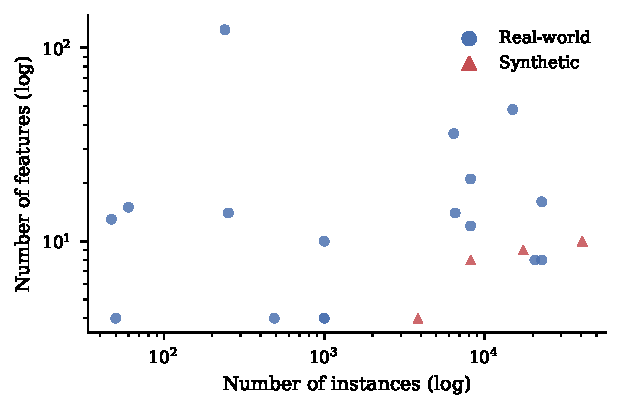
\includegraphics[width=0.62\textwidth]{figuras/fig_datasets.pdf}
\caption{Number of instances and number of features of the selected data sets (log scales).}
\label{fig:datasets}
\legend{Source: The Author}
\end{figure}

\section{Learning Algorithms and Implementation}
\label{sec:met-algoritmos}

The five algorithms described in Section~\ref{sec:fund-algoritmos} were used in
every scenario, through their scikit-learn implementations:
\texttt{LinearRegression} (LR), \texttt{KNeighborsRegressor} (KNN),
\texttt{DecisionTreeRegressor} (DT), \texttt{RandomForestRegressor} (RF), and
support vector regression (SVR). Outside the tuning scenario, all algorithms were
used with their default settings (for KNN, $k=5$ with the Euclidean distance;
for RF, 100 trees), and DT and RF received a fixed random seed so that differences between paired runs were not
caused by the randomness of tree construction.

Two implementation details concern SVR. First, because its regularization
parameter $C$ and its tolerance $\varepsilon$ are expressed in the scale of the
target, SVR was wrapped in a \texttt{TransformedTargetRegressor} that
standardizes the target inside each training fold and transforms predictions
back to the original scale before the metrics are computed; this transformation
is fitted only on training data in both pipelines and is therefore not a source
of leakage. Second, kernel SVR has a training cost that grows between
quadratically and cubically with the number of instances
\cite{chang2011}, which made it too slow for the largest data sets in the scenarios that do not
involve tuning. In the normalization, imputation, and
feature selection scenarios, SVR was thus trained with a linear model solved by
LIBLINEAR (\texttt{LinearSVR}, $C=1$, $\varepsilon=0.1$, $\varepsilon$-insensitive
loss) \cite{fan2008}, which optimizes the same objective as a linear-kernel SVR
at a cost that grows linearly with the data size. In the tuning scenario, in
which the kernel is one of the searched hyperparameters, the LIBSVM-based
\texttt{SVR} implementation was used.
% TODO (Vinicius): confirmar se as rodadas finais usaram os valores padrao das
% variaveis de ambiente (SVR_IMPL=linear, SVR_SCALE_Y=1, NUM_TRIALS=6) e se houve
% subamostragem do SVR (SVR_MAX_ROWS) no tuning. O texto acima assume os padroes.

\section{Leakage Scenarios}
\label{sec:met-cenarios}

The four scenarios are described below. Table~\ref{tab:cenarios} summarizes, for
each one, the validation protocol, the specific factor and its levels, and the
number of pairs obtained.

\begin{table}[htb]
\centering
\caption{Summary of the experimental setup of each leakage scenario.}
\label{tab:cenarios}
\small
\begin{tabular}{p{2.5cm}p{3.6cm}p{4.4cm}r}
\toprule
\textbf{Scenario} & \textbf{Validation} & \textbf{Specific factor (levels)} & \textbf{Pairs} \\
\midrule
Normalization & 6 $\times$ 4-fold CV & -- & 630 \\
Imputation & 6 $\times$ 4-fold CV & Imputer (mean, median, KNN) $\times$ missing rate (5, 10, 20, 30\%) & 7,560 \\
Feature selection & 6 $\times$ hold-out (80/20) & Percentile of features kept (1, 5, 10, 20\%) & 2,520 \\
Hyperparameter tuning & 6 $\times$ 4-fold CV (nested in the leakage-free pipeline) & -- & 630 \\
\bottomrule
\end{tabular}
\\[2pt]
\footnotesize Source: The Author. Pairs = 21 data sets $\times$ 5 algorithms $\times$ levels $\times$ 6 repetitions.
\end{table}

\subsection{Normalization}
\label{sec:met-normalizacao}

Features were standardized with the $z$-score transformation
(Equation~\ref{eq:zscore}), implemented by scikit-learn's
\texttt{StandardScaler}. In the leakage-free pipeline, the scaler is the first
step of a \texttt{Pipeline} object evaluated with $4$-fold CV, so that its means
and standard deviations are re-estimated on the three training folds of each
iteration. In the leakage-prone pipeline, the scaler is fitted once on the whole
data set, the standardized matrix is passed to the CV, and the pipeline evaluated
inside the CV has no scaling step. In each repetition $i$, both pipelines use the
same \texttt{KFold} partition (with shuffling and seed $i$), and the score of the
repetition is the average of the four test folds.

\subsection{Missing Value Imputation}
\label{sec:met-imputacao}

Since PMLB data sets are complete, missing values had to be introduced
artificially. To make the scenario closer to real data, a MAR mechanism was adopted, using
the masking procedure proposed by \citeonline{muzellec2020}, whose reference
implementation was adapted for this work. In this procedure, a random subset of
90\% of the features (at least one) is kept fully observed; each of the
remaining features receives missing values with probabilities given by a
logistic model of the observed features, whose random coefficients are
normalized and whose intercepts are adjusted so that the expected proportion of
missing entries in each affected feature equals the target missing rate. Four
rates were used: 5\%, 10\%, 20\%, and 30\%. The target column was never masked.
The incomplete data set is generated once per data set and missing rate, and is
shared by both pipelines and by all algorithms and imputers, so that every pair
sees exactly the same missing entries. Note that, by construction, only about
one tenth of the features are affected; for the many data sets with four to ten
features, this corresponds to a single incomplete feature.

Three imputers were compared: mean and median imputation
(\texttt{SimpleImputer}) and KNN imputation (\texttt{KNNImputer}, $k = 5$). In
the leakage-free pipeline, the imputer is the first step of the pipeline,
followed by the scaler and the regressor, and is refitted on the training folds
of each CV iteration. In the leakage-prone pipeline, the imputer is fitted and
applied to the complete incomplete matrix, after which the imputed data are
evaluated with the pipeline \emph{scaler $\rightarrow$ regressor}. As in the
normalization scenario, both pipelines are evaluated with the same $4$-fold
partitions in each of the six repetitions.

\subsection{Feature Selection}
\label{sec:met-selecao}

Feature selection was performed with a univariate filter, scikit-learn's
\texttt{SelectPercentile} with the $F$-statistic for regression
(\texttt{f\_regression}), keeping 1\%, 5\%, 10\%, or 20\% of the
highest-scoring features. These low percentiles were chosen on purpose: the fewer features are kept, the
more the result depends on the exact ranking of the features, and the more the
test instances can influence it.
Whenever a percentile would select less than one feature, it was raised to the
smallest value that keeps exactly one, and the same adjusted value was used in
both pipelines. As a consequence, the 1\% and 5\% levels keep a single feature in every
data set with up to 21 features, the data sets with four features keep a single
feature at all four levels, and only \texttt{505\_tecator} keeps more than one
feature at the 1\% level. Different levels may therefore correspond to the same
selection, a fact that must be considered when interpreting the results by level.

This scenario uses repeated hold-out instead of CV. In the leakage-prone
pipeline, the selector is fitted once on all instances, \emph{including their
target values}, and the reduced matrix is then split into training (80\%) and
test (20\%) sets. In the leakage-free pipeline, the split is made first and the
selector is fitted inside the pipeline on the training set only. In both cases
the pipeline continues with the scaler and the regressor, and the metrics are
computed on the predictions for the test set. Each of the six repetitions uses a
different random split (seed $i$), shared by both pipelines.

\subsection{Hyperparameter Tuning}
\label{sec:met-tuning}

Hyperparameters were tuned by exhaustive grid search (\texttt{GridSearchCV}).
The grids, listed in Table~\ref{tab:grades}, were kept small enough to make nested CV feasible on all data sets, but still
contain between four and fifteen
candidate configurations per algorithm. In the leakage-prone pipeline, a single
$4$-fold CV is used both to select the configuration and to report its
performance: for each metric, the reported value is the mean CV score of the
best configuration according to that same metric, which corresponds to the
common practice of reporting the best score found during the search. In the
leakage-free pipeline, the same search is embedded in a nested CV: the outer
$4$-fold CV, with exactly the same partitions as the leakage-prone pipeline,
provides the test folds, and an inner $4$-fold CV run on the training part of
each outer fold selects the configuration (by MSE), which is then refitted on
that training part and evaluated on the outer test fold. In both pipelines,
feature scaling is part of the pipeline being tuned.

\begin{table}[htb]
\centering
\caption{Hyperparameter grids used in the tuning scenario.}
\label{tab:grades}
\small
\begin{tabular}{lp{8.6cm}r}
\toprule
\textbf{Alg.} & \textbf{Grid} & \textbf{Configs.} \\
\midrule
LR  & \texttt{fit\_intercept} $\in$ \{True, False\}; \texttt{positive} $\in$ \{True, False\} & 4 \\
KNN & $k \in \{3, 5, 7, 9, 11\}$; distance $\in$ \{Euclidean, Manhattan\} & 10 \\
DT  & \texttt{max\_depth} $\in \{3, 5, 8, 10, \text{None}\}$ & 5 \\
RF  & \texttt{n\_estimators} $\in \{100, 200, 500\}$; \texttt{max\_depth} $\in \{3, 5, 8, 10, \text{None}\}$ & 15 \\
SVR & $C \in \{0.01, 0.1, 1, 10, 100\}$; kernel $\in$ \{linear, RBF\} & 10 \\
\bottomrule
\end{tabular}
\\[2pt]
\footnotesize Source: The Author
\end{table}

\section{Effect Measures and Statistical Analysis}
\label{sec:met-analise}

The four metrics of Section~\ref{sec:fund-regressao} were recorded for every
run. The analysis concentrates on $R^2$, which is comparable across data sets,
and uses RMSE as a complementary measure. For each pair, the effect of leakage is
quantified by
\begin{equation}
  \Delta R^2 = R^2_{\text{leak}} - R^2_{\text{no leak}}
  \qquad \text{and} \qquad
  \Delta\text{RMSE} = 100 \times \frac{\text{RMSE}_{\text{no leak}} - \text{RMSE}_{\text{leak}}}{\text{RMSE}_{\text{no leak}}}\;(\%).
  \label{eq:deltas}
\end{equation}
Both measures are oriented so that a \emph{positive} value means that leakage
made the model look better than it is: a higher $R^2$ or a lower RMSE. $\Delta$RMSE
is expressed as a percentage of the leakage-free RMSE to remove the dependence on
the scale of the target. A pair is considered a tie when
$\lvert \Delta R^2 \rvert \leq 10^{-9}$, a tolerance that absorbs floating-point
noise; the proportions of pairs in which leakage improved, did not change, or
worsened the estimate are reported for each scenario and algorithm.

Statistical tests follow the recommendations of \citeonline{demsar2006} and use
the data set as the unit of analysis. For each scenario and algorithm, the
$\Delta R^2$ of all pairs of a data set (across repetitions and levels of the
specific factor) are averaged, producing 21 values, one per data set. The
two-sided Wilcoxon signed-rank test is applied to these values to test whether
the median effect differs from zero, and the five $p$-values of each scenario
(one per algorithm) are adjusted with the Holm procedure. Results are considered
significant at $\alpha = 0.05$ after adjustment. Testing each configuration separately would be less informative, since with six
pairs the smallest possible two-sided $p$-value is $0.031$; at that level, the number of configurations in
which leakage improved the estimate in all six repetitions is reported instead,
as a descriptive measure of consistency.

To answer RQ3, the Friedman test is applied, in each scenario, to the
per-data-set mean $\Delta R^2$ of the five algorithms, testing whether some
algorithms are systematically more affected than others. To answer RQ4, the
Spearman correlation is computed between the per-data-set mean $\Delta R^2$
(averaged over algorithms) and the number of instances ($n$), the number of
features ($d$), and the ratio $d/n$. The analysis scripts were written in Python
with pandas and SciPy, and all numbers reported in Chapter~\ref{cap:resultados}
are produced by the script \texttt{tcc/scripts/gerar\_tabelas\_figuras.py}
directly from the raw result files.

% Capitulos 5 e 6 ainda em construcao. Mantidos apenas como marcadores para
% que as referencias cruzadas dos capitulos 1 a 4 nao aparecam como "??".
\chapter{Results and Discussion}
\label{cap:resultados}

\emph{This chapter is under construction.}

\chapter{Conclusion}
\label{cap:conclusao}

\emph{This chapter is under construction.}


% -------------------- Referencias --------------------
\bibliographystyle{abntex2-alf}
\bibliography{referencias}


\end{document}
